\documentclass{article}
\usepackage{hyperref}
\usepackage{graphicx}

\begin{document}


\title{Resequencing against a sequence variation graph}

\author{Erik Garrison}

\maketitle

\begin{abstract}
Despite the availability of whole genome sequences from many individuals in many species, when examining a new genome we only use single reference haplotype as our basis for interpretation. As a result, our analyses are biased against the detection of any variation comprising significant differences from this reference haplotype. To resolve this issue, and also to expand resequencing approaches to organisms for which no single reference sequence has been (or can be) constructed, we propose the use of sequence graphs that simultaneously describe all known genomes. We first outline the basic model. Then, we describe its implementation in a reusable software library.
\end{abstract}

\section{Introduction}

Where genomes are small and sequences from different individuals can be reliably isolated, we can understand variation by assembling whole genomes and then comparing them via whole-genome comparison approaches \cite{mummer}.
However, as the genomes of organisms of interest (such as \emph{Homo sapiens}) are often large \cite{pmid11237011}, and the genomes of organisms we want to understand are often complex and difficult to completely assemble reliably using existing technology (for example, that of \emph{Plasmodium falciparum} still contains 80 gaps \cite{pfalciparum, pfalciparumweb}), standard practice involves the localization of short reads against a single high-quality reference system that is typically composed of a single haplotype per homologous region. Conceptually, this reference describes a single hypothetical individual, although in practice sequences from many individuals may be used to generate the assembly.

\subsection{Resequencing against a linear reference system}

In \emph{resequencing}, we use alignments against a set of reference sequences (typically chromosomes or assembly contigs) to describe variation in a new sample. By linking new observations into a common reference system, resequencing provides a coherent approach to relate the genomes of individuals in an entire population. However, as this approach requires sufficient similarity between variant sequences in order to relate them, we may be unable to directly observe many kinds of variation, such as large insertions and deletions of sequence (indels) or even clusters of smaller variation (such as single nucleotide polymorphisms, SNPs). Indels, which contribute significantly to sequence diversity \cite{mills2010}, are particularly difficult, in that sequences derived from insertions relative to the reference sequence cannot be easily localized against the reference. This contributes significantly to the difficulty of genotyping transposable element insertion polymorphisms, which are still poorly-understood despite the efforts of large-scale sequencing projects \cite{stewart2011}. Similarly, copy-number variations, which influence large regions of the human genome, are difficult to genotype in new samples even when previously-known \cite{sudmant2010}.

Although these problems are more general than the specific resequencing informatics techniques that are applied, in all cases the basic problem is that cost of discovery of novel variation is equivalent to the cost of genotyping known variation in a new sample. However, this effort seems wasted, as most variation is shared, particularly in species with relatively small effective population sizes such as humans. Resources such as that produced by the 1000 Genomes Project now contain the vast majority (greater than $95\%$) of variation that we expect to find in a newly-sequenced human individual \cite{1000Gphase1}. If we could generate a reference system including this variation, we could reduce the cost of genotyping it in new samples. We now describe a basic model for such a system and the implementation of data formats and a software library designed to enable resequencing approaches to operate against this generalize reference system.

\begin{figure}[h!]
\centering
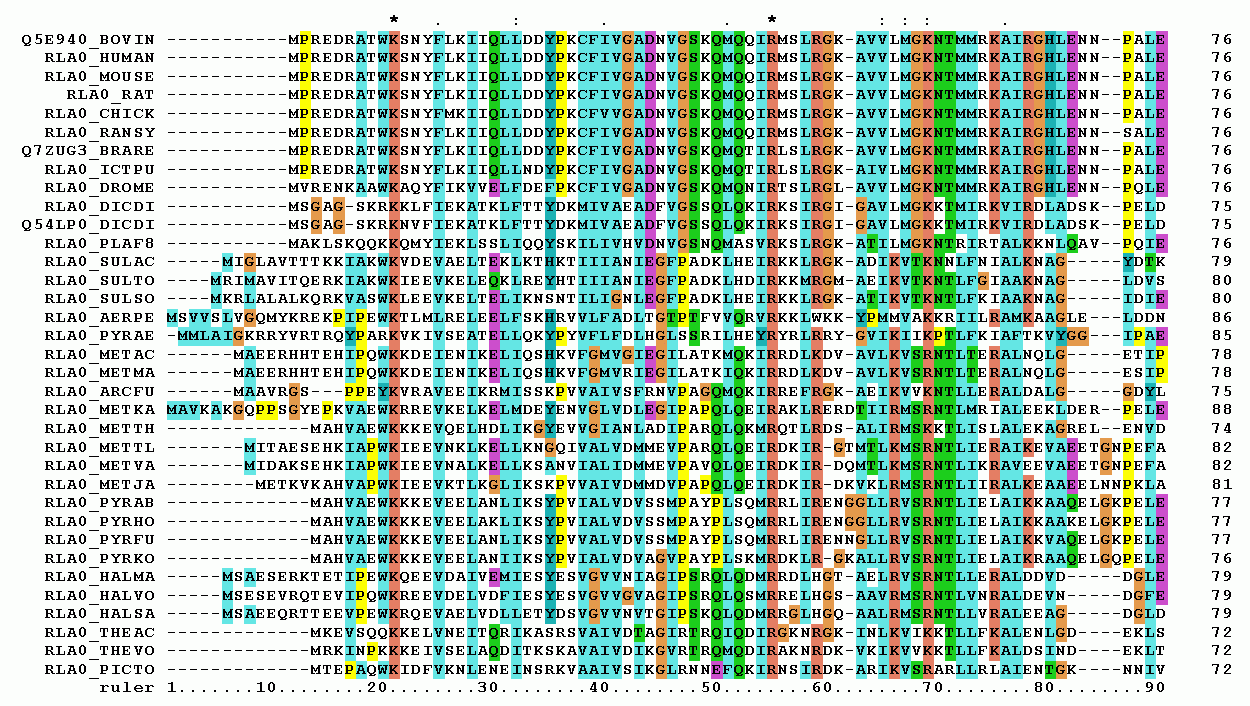
\includegraphics[width=1.0\textwidth]{figures/RPLP0_90_ClustalW_aln}
\caption{\label{fig:msa}
  First 90 positions of a protein multiple sequence alignment of instances of the acidic ribosomal protein P0 (L10E) from several organisms. Generated with ClustalX. Credit: Miguel Andrade \url{https://commons.wikimedia.org/wiki/File:RPLP0_90_ClustalW_aln.gif}. CC BY-SA 3.0.
}
\end{figure}

\subsection{Partially-ordered sequence graphs}

A traditional model to combine variation from many samples into one reference system is the multiple sequence alignment (\hyperref[fig:msa]{figure \ref{fig:msa}}). In this approach, sequences are encoded using an additional gap character, typically represented as ``-'', which indicates when one sequence in the multiple sequence alignment (MSA) has additional sequence where the one in which the gap is included does not. This mutually-gapped alignment has the desirable property that it fully-represents all of the sequences which were mutually aligned. This model has a dual representation as a partially-ordered graph in which nodes contain sequences in the alphabet of allowed characters (A, C, G, T for DNA, or the amino acids codes for proteins). In this partially-ordered graph, homologous aligned sequences are compressed into a single node or series of nodes (\hyperref[fig:poa]{figure \ref{fig:poa}}). Generalizations of pairwise alignment \cite{gotoh1982} allow the alignment of new sequences directly to this structure in $O(NM)$ time, where $N$ is the length of the query and $M$ the sum of lengths of unique sequences in the partially-ordered sequence graph \cite{lee2002POA}.

\begin{figure}[h!]
\centering
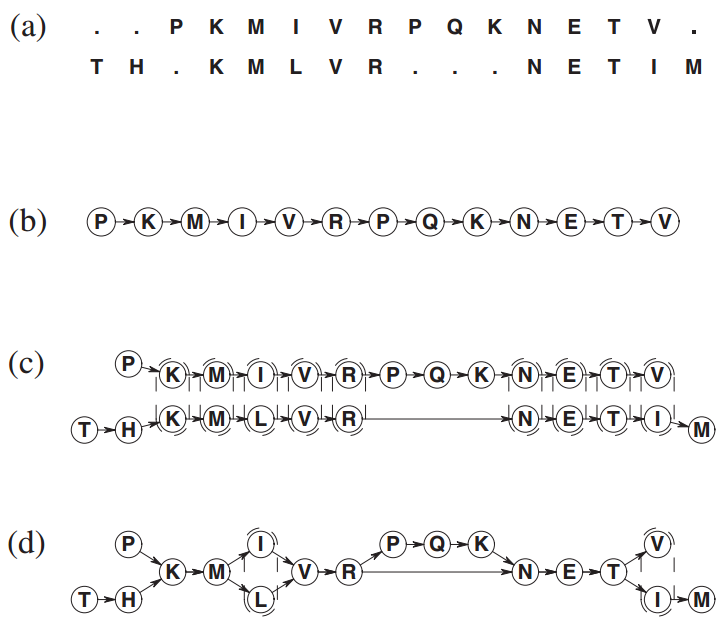
\includegraphics[width=0.8\textwidth]{figures/poamsa}
\caption{\label{fig:poa}
The relationship between a multiple sequence alignment (MSA) and a partially-ordered sequence graph (POA). (a) A gapped MSA representation for a pairwise protein alignment. (b) A single sequence in POA format. (c) The alignment of two sequences in POA format. (d) The POA representation of the original MSA. From \cite{lee2002POA}.
}
\end{figure}


\begin{figure}
\centering
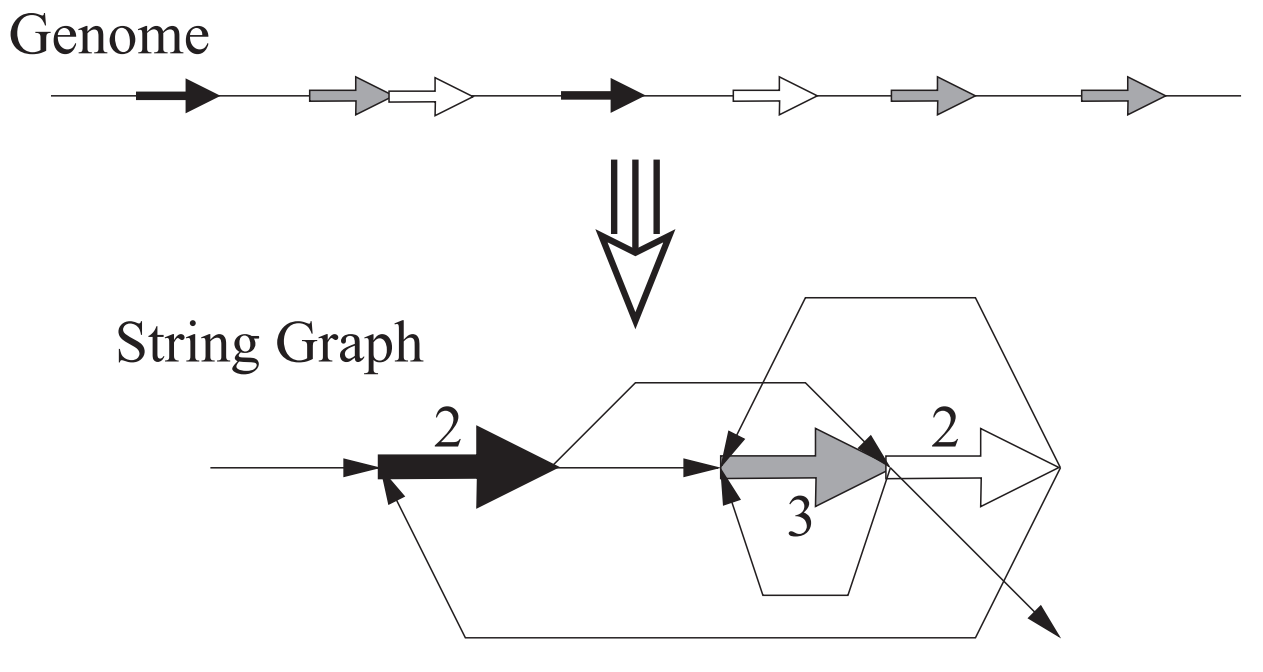
\includegraphics[width=1.0\textwidth]{figures/stringgraph}
\caption{\label{fig:stringgraph}
A genome and its string graph. Thick arrows illustrate identical, repeated sequences. Numbers describe copy-number counts. Edges represent linkages observed in shotgun sequencing data from the genome. From \cite{myers2005}.
}
\end{figure}

\subsection{Assemblies using string graphs and de Bruijn graphs}

While the partially-ordered representation of sequence variation can provide full information of many related sequences in a single model, the requirement of partial ordering limits its use to contexts where the complete synteny of a particular region can be established. A more general model for representing many sequences in the same context and allowing for cycles is the string graph, which was proposed by \cite{myers2005} and implemented efficiently at scale by \cite{simpson2010} in the SGA assembler. This represention captures and compresses all information about a genome or collection of genomes that can be derived from shotgun sequencing results (\ref{fig:stringgraph}). Sequences which are repeated in the input, such as transposons or copy number amplifications, are compressed into a single node in the string graph. The string graph does not require order, although it should be noted that it exhibits a manifold property in that small neighborhoods of the graph may maintain partial order. This property allows local alignment using methods described against partial orders, and further extensions of such methods allow alignment of cyclic graphs to cyclic graphs \cite{myers1988}.

A similar approach to representing the sequences in a shotgun sequencing experiment in the same context is the de Bruijn graph. In this structure, each node represents a sequence of fixed size (a k-mer), and edges occur between nodes where the relationship $n_i[1,\ldots,k] = n_j[0,\ldots,k-1]$ is satisfied. This structure has certain advantages conceptually over string graphs, in that it is often easier to operate on fixed-size kmers. However, as each novel k-mer in the graph will generate a series of new nodes, methods must prune the graph by filtering low-frequency sequences \cite{iqbal}. The lossy nature of practical implementations of this structure makes it less-attractive as a target model for representing many samples at the same time.

\subsection{Reference genome structures}

Recent work \cite{paten2014} describes a comprehensive system that is related in scope to both string graphs and partially-ordered sequence graphs. In this \emph{reference genome structure}, sequences are attached to nodes and linkages between sequences occur where two sequences were observed in synteny in some haplotype in a reference set. This structure extends on other forms of sequence graphs by adding a mapping operation to the graph. In this \emph{left-right mapping} operation, the mapping of a new sequence (or more generally, another graph) into the existing reference system is driven by the discovery of unique contexts of a given length surrounding each node or neighborhood in the graph.

\subsection{Sequence variation graphs}

In this effort, we sought to develop a practical implementation of a reference system that can (1) be used to represent and describe variation in many related samples (such as from the same species), (2) allow mapping of new sequences into this space, and (3) enable the genotyping (effectively copy-number assignment) of segments in the graph in a given individual or set of individuals whose sequencing results have been mapped into the system. These requirements may be met by a number of underlying representations, but for the sake of expediency, we have chosen to implement first a generic model which places no restrictions on the structure of the graph. For instance, we do not require that repeated sequences are represented only once (as in string graphs), or that mappings require particularly-sized globally-unique contexts (as in reference genome structures). Nor is there a particular limit placed on the size of nodes. In a global context we allow for cycles, but when mapping we require the graph is partially ordered. This \emph{sequence variation graph} is simply a general, assumption-free model that allows us to begin building a practical system to enable resequencing against both genome assemblies (e.g. string graphs) and partial orders such as are implied by a reference genome and a VCF file.

\section{Methods}

Formally, our model is a graph $G$ comprised of a set of nodes $N = n_1, \ldots ,n_M$ and a set of edges $E = e_1, \ldots, e_L$ such that $|N| = M$ and $|E| = L$. Each node $n_i$ represents a sequence $s_i$ which is built from an arbitrary alphabet $l$. For DNA sequences, we might use $l = \{ A, T, G, C, N \}$, but in principle the model can be based in any alphabet. Edges represent linkages between sequences that have been observed in a reference set of samples.



\section{Results}

\section{Discussion}

\bibliography{references}{}

\bibliographystyle{plain}




\end{document}
